\documentclass[aspectratio=169]{beamer}
\usetheme{Madrid}
\usecolortheme{beaver}
\usepackage[utf8]{inputenc}
\usepackage[T1]{fontenc}
\usepackage{tikz}
\usepackage{amssymb}
\usepackage{graphicx}
\setbeamertemplate{navigation symbols}{}
\setbeamercolor{title}{fg=white,bg=cyan!60!black}
\setbeamercolor{frametitle}{fg=white,bg=cyan!50!black}
\setbeamercolor{block title}{bg=cyan!15,fg=black}
\setbeamercolor{block body}{bg=cyan!5,fg=black}

\title{G5 — Player Control}
\subtitle{Keyboard + mouse input schemes, aiming}
\author{ByteForge --- Grade 7 --- Game Maker --- Week Overview}
\date{}

\begin{document}

\begin{frame}
    \titlepage
\end{frame}

\begin{frame}{This Week's Plan}
    \begin{itemize}
        \item Lesson 1: Move with Arrow Keys
        \item Lesson 2: Aim with the Mouse
        \item Lesson 3: Two-Player Split
        \item[$\bigstar$] BOSS --- Top-Down Shooter Controls (\texttt{lessonBoss.tex})
    \end{itemize}
\end{frame}

\begin{frame}{Real-World Example}
    \Large
    A split-screen couch co-op game (two controllers, two characters on one screen) is exactly this chapter's "two independent input schemes, one frame loop" idea, running in a real shipped game. Minecraft moves with WASD (keyboard) while the mouse independently aims/looks around — the exact keyboard+mouse split this chapter teaches.
\end{frame}


\begin{frame}{Image}
    \begin{center}
    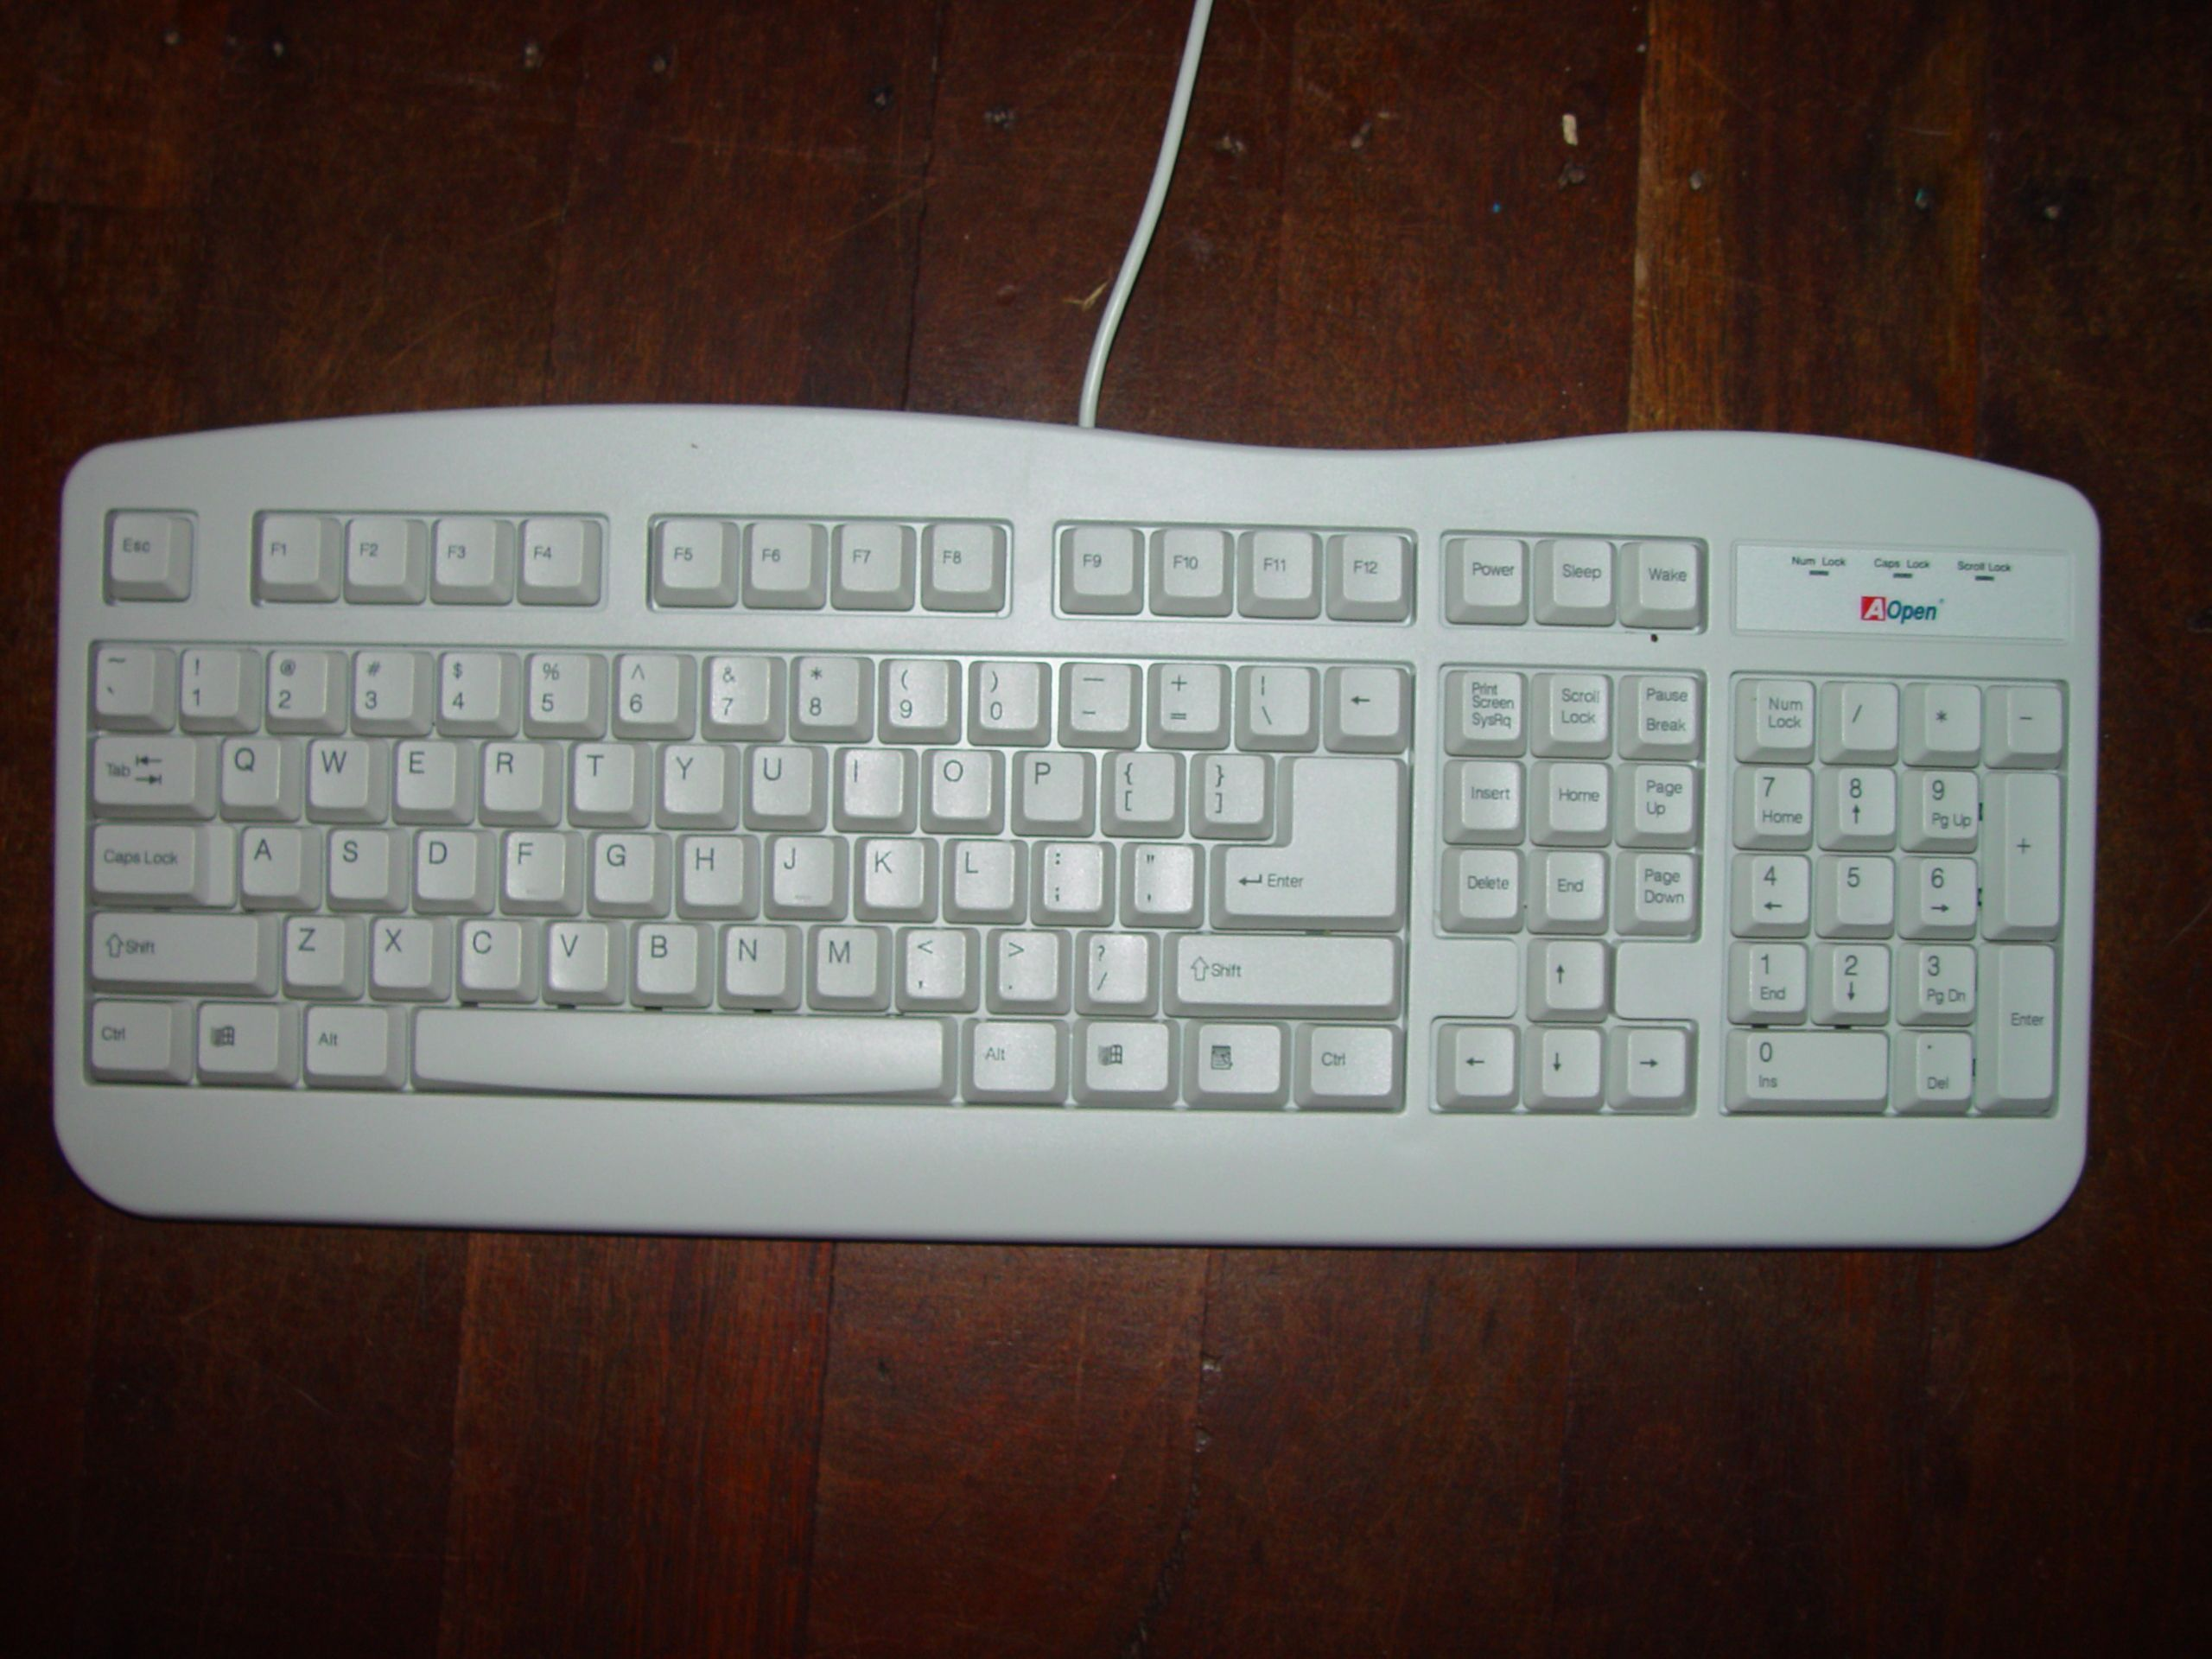
\includegraphics[width=0.55\textwidth]{../images/keyboard.jpg}

    \small Computer keyboard, public domain, via Wikimedia Commons
    \end{center}
\end{frame}

\begin{frame}{Let Them Discover}
    \Large
    Play any game with both keyboard movement AND mouse aiming (Minecraft included). Try to notice: does moving affect aiming, or are they genuinely independent? What would break if they shared one set of variables?
\end{frame}

\begin{frame}{Files in This Folder}
    \small
    \begin{itemize}
        \item \texttt{lesson1.tex} --- Move with Arrow Keys
        \item \texttt{lesson2.tex} --- Aim with the Mouse
        \item \texttt{lesson3.tex} --- Two-Player Split
        \item \texttt{lessonBoss.tex} --- BOSS: Top-Down Shooter Controls
    \end{itemize}
    \vspace{0.5em}
    \normalsize Each lesson file is its own short deck --- open the one for
    the specific day you're teaching, not this whole overview.
\end{frame}

\end{document}
